\documentclass[12pt]{article}
\usepackage[utf8]{inputenc}
\usepackage[english]{babel}
\usepackage[letterpaper,top=2cm,bottom=2cm,left=3cm,right=3cm,marginparwidth=1.75cm]{geometry}
\usepackage{amsmath}
\usepackage{tikz}
\usepackage{graphicx}
\usepackage{bigints}
\usepackage{amssymb}
\usepackage[colorlinks=true, allcolors=blue]{hyperref}

\setlength\parindent{0pt}
\DeclareMathOperator{\vol}{vol}
\newcommand{\RR}{\mathbb{R}}
\newcommand{\inv}{^{-1}}
\newcommand{\pder}[2]{\frac{\partial #1}{\partial #2}}

\title{Math 31CH HW3 SOLUTIONS \\ Due April 19 at 11:59 pm by Gradescope Submission}
\author{Professor Bennett Chow}
\date{}

\begin{document}
\maketitle



\begin{center}
   \textbf{EXERCISES FOR SECTION 4.9}
\end{center}

\textcolor{red}{Exercise 4.9.1:}
Let $T:\RR^n\to \RR^n$ be given by the matrix
\begin{equation*}
    \begin{bmatrix}
    1 & 0 & 0 & \cdots & 0 \\
    2 & 2 & 0 & \cdots & 0 \\
    3 & 3 & 3 & \cdots & 0 \\
    \vdots  & \vdots & \vdots & \ddots & \vdots \\
    n & n & n & \cdots & n \\
    \end{bmatrix} ,
\end{equation*}
and let $A \subset \RR^n$ be the region given by
\begin{equation*}
    |x_1| +|x_2|^2 +|x_3|^3 +\cdots+ |x_n|^n \leq 1.
\end{equation*}
What is $\operatorname{vol}_n T(A) / \operatorname{vol}_n A$?\smallskip

\textcolor{blue}{Solution to 4.9.1:}
The fraction can be calculated using the determinant of $T$,
which ends up being the product of the diagonal entries.
\[
    \frac{\vol_n T(A)}{\vol_n A} = \det T = n!
\]
\newpage


\textcolor{red}{Exercise 4.9.4:}
What is the $n$-dimensional volume of the region
\begin{equation*}
    \big\{ \mathbf{x}\in \RR^n \, | \, x_i \geq 0 \text{ for all } i=1,\ldots,n \text{ and } x_1+\cdots + x_n \leq 1 \big\} \,?
\end{equation*}

\textcolor{blue}{Solution to 4.9.4:}
Let $V_n(t)$ represent the volume of the region 
$S_n(t) = \big\{ \mathbf{x}\in \RR^n \, | \, x_i \geq 0 \text{ for all } i=1,\ldots,n \text{ and } x_1+\cdots + x_n \leq t \big\}$.
Therefore, 
\begin{align*}
    V_n(1) 
    &= \int_{S_n(1)} |d^n x| \\
    &= \int _0^1 V_{n-1}(1-x_n) \,dx_n \\
    &= \int _0^1 (1-x_n)^{n-1} V_{n-1}(1) \,dx_n \\
    &= V_{n-1}(1) \left[ -\frac{1}{n} (1-x_n)^n \right]_0^1 \\
    &= \frac{1}{n} V_{n-1}(1)
\end{align*}
Since $V_1(1) = 1$, by induction we have that $V_n(1) = \frac{1}{n!}$.
\newpage

\textcolor{red}{Exercise 4.9.6:}
Compute the volume of the three $k$-parallelograms ($k=3,4,5$) spanned by the vectors:

(a)
\begin{equation*}
    \begin{bmatrix}
    1\\3\\-1
    \end{bmatrix} , \;
        \begin{bmatrix}
    2\\-1\\-1
    \end{bmatrix} , \;
        \begin{bmatrix}
    3\\6\\0
    \end{bmatrix} .
\end{equation*}

(b)
\begin{equation*}
    \begin{bmatrix}
    1\\1\\1\\0
    \end{bmatrix} , \;
    \begin{bmatrix}
    1\\1\\0\\1
    \end{bmatrix} , \;
        \begin{bmatrix}
    1\\0\\1\\1
    \end{bmatrix} , \;
        \begin{bmatrix}
    0\\1\\1\\1
    \end{bmatrix} .
\end{equation*}

(c)
\begin{equation*}
    \begin{bmatrix}
    4\\3\\2\\1\\0
    \end{bmatrix} , \;
    \begin{bmatrix}
    3\\2\\1\\0\\1
    \end{bmatrix} , \;
    \begin{bmatrix}
    2\\1\\0\\1\\2
    \end{bmatrix} , \;
    \begin{bmatrix}
    1\\0\\1\\2\\3
    \end{bmatrix} , \;
    \begin{bmatrix}
    0\\1\\2\\3\\4
    \end{bmatrix} .
\end{equation*}

\textcolor{blue}{Solution to 4.9.6:}
The volumes of the parallelograms can be calculated 
by taking the absolute value of the determinant.
\begin{enumerate}
    \item 
        The volume is 18.
        \[
        \det 
        \begin{bmatrix}
            1 & 2 & 3 \\
            3 & -1 & 6 \\
            -1 & -1 & 0
        \end{bmatrix} 
        = 1(6)-2(6)+3(-4)
        =-18
        \]
        
    \item 
        The volume is 3.
        \[
        \det 
        \begin{bmatrix}
            1 & 1 & 1 & 0 \\
            1 & 1 & 0 & 1 \\
            1 & 0 & 1 & 1 \\
            0 & 1 & 1 & 1
        \end{bmatrix}
        = 1(-1) - 1(1) +1(-1)
        = -3
        \]
    \item 
        The volume is 32.
        \[
        \det 
        \begin{bmatrix}
            4 & 3 & 2 & 1 & 0 \\
            3 & 2 & 1 & 0 & 1 \\
            2 & 1 & 0 & 1 & 2 \\
            1 & 0 & 1 & 2 & 3 \\
            0 & 1 & 2 & 3 & 4
        \end{bmatrix}
        =4(4) - 3(0) + 2(0) - 1(-16)
        = 32
        \]     
\end{enumerate}


\newpage

\begin{center}
   \textbf{EXERCISES FOR SECTION 4.10}
\end{center}

\textcolor{red}{Exercise 4.10.4:}
Use the change of variables formula to compute the volume of the region
\begin{equation*}
    \frac{x^2}{(z^3-1)^2} + \frac{y^2}{(z^3+1)^2} \leq 1, \quad -1\leq z\leq 1 ,
\end{equation*}
shown in the Figure on p.~497.\medskip

\textcolor{blue}{Solution to 4.10.4:}
Horizontal slices of the figure are ellipses, so we can use the map
\[
    \Phi\begin{pmatrix} r \\ \theta \\ z\end{pmatrix} \to 
    \begin{pmatrix}
        (z^3-1)r\cos \theta \\
        (z^3+1)r\sin \theta \\
        z \\
    \end{pmatrix}
\]
The determinant of the Lipschitzs derivative is 
\begin{align*}
    \det 
    \begin{bmatrix}
        \pder{x}{r} & \pder{x}{\theta} & \pder{x}{z} \\
        \pder{y}{r} & \pder{y}{\theta} & \pder{y}{z} \\
        \pder{z}{r} & \pder{z}{\theta} & \pder{z}{z} \\
    \end{bmatrix} 
    &= \det 
    \begin{bmatrix}
        (z^3-1)\cos \theta & -(z^3-1)r\sin \theta &  3z^2r\cos \theta\\
        (z^3+1)\sin \theta & (z^3+1)r\cos \theta & 3z^2r\sin \theta \\
        0 & 0 & 1 \\
    \end{bmatrix} \\
    &= 0 - 0 + 1((z^6-1)r\cos^2\theta + (z^6-1)r\sin^2\theta) \\
    &= (z^6-1)r
\end{align*}
Therefore the integral is given by 
\begin{align*}
    \int_0^{2\pi} \int_0^1 \int_{-1}^1 |(z^6-1)r| \,dz \,dr \,d\theta
    &= \int_0^{2\pi} \int_0^1  \frac{12}{7}r \,dr \,d\theta \\
    &= \int_0^{2\pi} \frac{6}{7} \,d\theta \\
    &= \frac{12}{7} \pi
\end{align*}
\newpage

\textcolor{red}{Exercise 4.10.5:} (a) What is the area of the ellipse $x^2/a^2 + y^2 /b^2 \leq 1$? \emph{Hint}: Use the change of variables $u=x/a$, $v=y/b$.

(b) What is the volume of the ellipsoid $x^2/a^2 + y^2 /b^2 + z^2/c^2 \leq 1$?
\medskip

\textcolor{blue}{Solution to 4.10.5:}
\begin{enumerate}
    \item The following parameterization maps from the unit circle to the ellipse.
        \[
            \Phi\begin{pmatrix} u \\ v \end{pmatrix} \to 
            \begin{pmatrix}
                au \\
                bv
            \end{pmatrix}
        \]
        The determinant of the Lipschitzs derivative is $ab$, meaning it streches
        the area of the unit circle by $ab$ to get the area of the ellipse.
        Therefore the area of the ellipse is $\pi ab$.
    \item The following parameterization maps from the unit sphere to the ellipsoid.
        \[
            \Phi\begin{pmatrix} u \\ v \\ w\end{pmatrix} \to 
            \begin{pmatrix}
                au \\
                bv \\
                cw 
            \end{pmatrix}
        \]
        The determinant of the Lipschitzs derivative is $abc$, 
        so the volume of the ellipsoid is $\frac{4}{3}\pi abc$.
\end{enumerate}



\newpage

\textcolor{red}{Exercise 4.10.8:} (a) For fixed $a,b>1$, let $U_{a,b}$ be the plane region in the first quadrant defined by the inequalities $1\leq xy \leq a$,
$x\leq y \leq bx$. Sketch $U_{2,4}$.

(b) Compute $\displaystyle \int_{U_{a,b}} x^2 y^2 \, |dx\, dy|$.
\medskip

\textcolor{blue}{Solution to 4.10.8:}
\begin{figure}[ht!]
    \centering
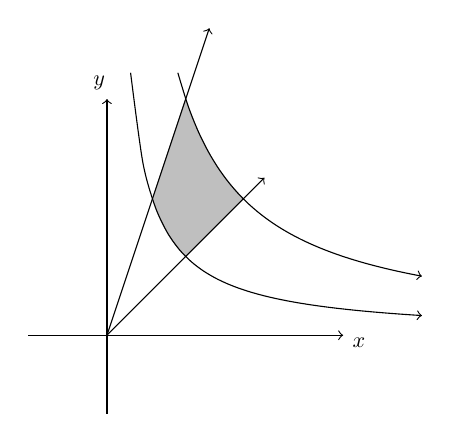
\begin{tikzpicture}
\filldraw[gray!50] plot[smooth,domain=0.58:1] (\x, {1/\x}) -- (1.73, 1.73);
\filldraw[gray!50] (0.58, 1.73) -- plot[smooth,domain=1:1.73] (\x, {3/\x}) -- (1,1);
\draw[->] (-1,0) -- (3,0) ;
\draw[->] (0,-1) -- (0,3) ;
\draw[->] plot[smooth,domain=0.3:4] (\x, {1/\x});
\draw[->] plot[smooth,domain=0.9:4] (\x, {3/\x});
\draw[->] plot[smooth,domain=0:2] (\x, {\x});
\draw[->] plot[smooth,domain=0:1.3] (\x, {3*\x});
\node[scale=.8] at (3.2,-.1) {$x$} ;
\node[scale=.8] at (-.1,3.2) {$y$} ;
\end{tikzpicture}
    \caption{Exercise 4.10.8.a}
\end{figure}

Using the change of variables $u = xy$ and $v = \frac{y}{x}$,
the parameterization is 
\[
    \Phi\begin{pmatrix} u \\ v\end{pmatrix} \to 
    \begin{pmatrix}
        \sqrt{\frac{u}{v}} \\ 
        \sqrt{uv}
    \end{pmatrix}
\]
The determinant of the Lipschitzs derivative is 
\begin{align*}
    \det 
    \begin{bmatrix}
        \pder{x}{u} & \pder{x}{v} \\ 
        \pder{y}{u} & \pder{y}{v}
    \end{bmatrix} 
    &= \det 
    \begin{bmatrix}
        \frac{1}{2\sqrt{uv}} &  -\frac{1}{2} \sqrt{\frac{u}{v^3}}\\ 
        \frac{1}{2}\sqrt{\frac{v}{u}} & \frac{1}{2}\sqrt{\frac{u}{v}}
    \end{bmatrix} \\
    &= \frac{1}{4v} + \frac{1}{4v} \\
    &= \frac{1}{2v}
\end{align*}
The integral is 
\[
    \int_1^a \int_1^b \frac{u^2}{2v} \,dv \,du
    = \int_1^a \frac{u^2}{2}\ln b \,du
    = \frac{\ln b}{6}(a^3-1)
\]
\newpage

\textcolor{red}{Exercise 4.10.12:}
Evaluate the iterated integral
\begin{equation*}
    \int_{-2}^2 \int_0^{\sqrt{4-x^2}} \int_0^{\sqrt{4-x^2-y^2}}
    (x^2 + y^2 +z^2)^{3/2} dz\,dy\,dx .
\end{equation*}


\textcolor{blue}{Solution to 4.10.12:}
Using spherical coordinates, the integral over the quarter-sphere becomes
\[
    \int_0^{\pi} \int_0^2 \int_0^{\frac{\pi}{2}}  
        r^5 \cos \varphi
        |\,d\varphi \,dr \,d\theta|
    = \pi \int_0^2 
        r^5
        \,dr 
    = \frac{32}{3}\pi
\]

\newpage

\textcolor{red}{Exercise 4.10.17:}
Let $Q_a=[0,a]\times [0,a]\subset \RR^2$ be the square of side length $a$ in the first quadrant, with two sides on the axes, and let $\Phi:\RR^2\to\RR^2$ be given by
\begin{equation*}
    \Phi \begin{pmatrix}
    u\\v
    \end{pmatrix} = \begin{pmatrix}
    u-v\\e^u+e^v
    \end{pmatrix} .
\end{equation*}
Set $A=\Phi(Q_a)$.

(a) Sketch $A$, by computing the image of each of the sides of $Q_a$.
It might help to being by drawing carefully the curves of
the equations $y=e^{x}+1$ and $y=e^{-x}+1$.

(b) Show that $\Phi : Q_a \to A$ is one-to-one.

(c) What is $\displaystyle \int_A y \, |dx\,dy|$\,?
\medskip

\textcolor{blue}{Solution to 4.10.17:}
\begin{figure}[ht!]
    \centering
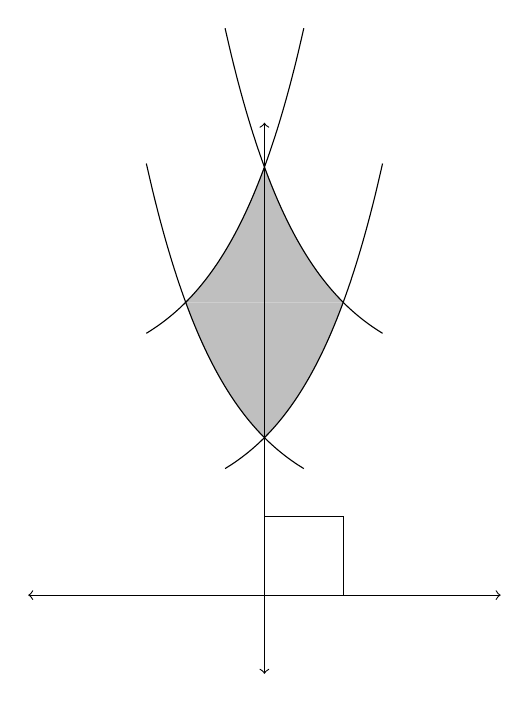
\begin{tikzpicture}
\draw (0,1) -- (1,1) -- (1,0);
\filldraw[gray!50] plot[smooth,domain=-1:0] (\x, {e^(-\x)+1}) -- plot[smooth,domain=0:1] (\x, {e^\x+1});
\filldraw[gray!50] plot[smooth,domain=-1:0] (\x, {e^(\x+1)+e}) -- plot[smooth,domain=0:1] (\x, {e^(1-\x)+e});

\draw plot[smooth,domain=-0.5:1.5] (\x, {e^\x+1});
\draw plot[smooth,domain=-1.5:0.5] (\x, {e^(-\x)+1});
\draw plot[smooth,domain=-1.5:0.5] (\x, {e^(\x+1)+e});
\draw plot[smooth,domain= -0.5:1.5] (\x, {e^(1-\x)+e});
\draw[<->] (-3,0) -- (3,0) ;
\draw[<->] (0,-1) -- (0,6) ;
\end{tikzpicture}
    \caption{Exercise 4.10.17.a}
\end{figure}

Assume that $\Phi$ is not one-to-one.
Therefore there exists different $(u_1, v_1)$ and $(u_2, v_2)$ such that 
$u_1-v_1 = u_2 - v_2$. 
So either $u_1 > u_2$ and $v_1 > v_2$ or $u_2 > u_1$ and $v_2 > v_1$.
However since $e^x$ is a strictly increasing function, 
$e^{u_1}+e^{v_1} = e^{u_2}+e^{v_2}$ cannot be true.
Therefore $\Phi$ must be one-to-one.

The determinant of the Lipschitzs derivative is 
\[
    \det 
    \begin{bmatrix}
        \pder{x}{u} & \pder{x}{v} \\
        \pder{y}{u} & \pder{y}{v}
    \end{bmatrix} =
    \det 
    \begin{bmatrix}
        1 & -1 \\
        e^u & e^v
    \end{bmatrix} =
    e^u + e^v
\]
Therefore the integral over $A$ is
\[
    \int_A y \, |dx\,dy|
    = \int_0^a \int_0^a (e^u + e^v)^2\,|du\,dv|
    = a(e^{2a}-1) + 2(e^a-1)^2
\]
\end{document}
